\documentclass{article}

\usepackage{titlesec}
\usepackage{graphicx}
\usepackage{subcaption}
\usepackage{wrapfig}
\usepackage{caption}
\usepackage[
backend=biber,
style=alphabetic,
sorting=ynt
]{biblatex}

\addbibresource{bibliography.bib} 

\titleformat{\section}[block]{\filcenter\Large\bfseries}{}{1em}{}
\captionsetup[figure]{labelformat=empty}

\title{Gibson ES-150}
\author{Ivan Dario Gonzalez Collazos}
\date{Febrero 28 del 2023}

\begin{document}

\maketitle

\section{Antecedentes}

Los intentos de crear una guitarra amplificada capturando el sonido por medio de un sistema eléctrico, se remontan desde la década de 1890, donde en diciembre de 1892 se registra la patente a nombre de W.H. Gilman que describe un banjo accionado automáticamente de manera eléctrica.\\

\begin{figure}[h]
    \begin{center}
        \begin{subfigure}{0.3\textwidth}
            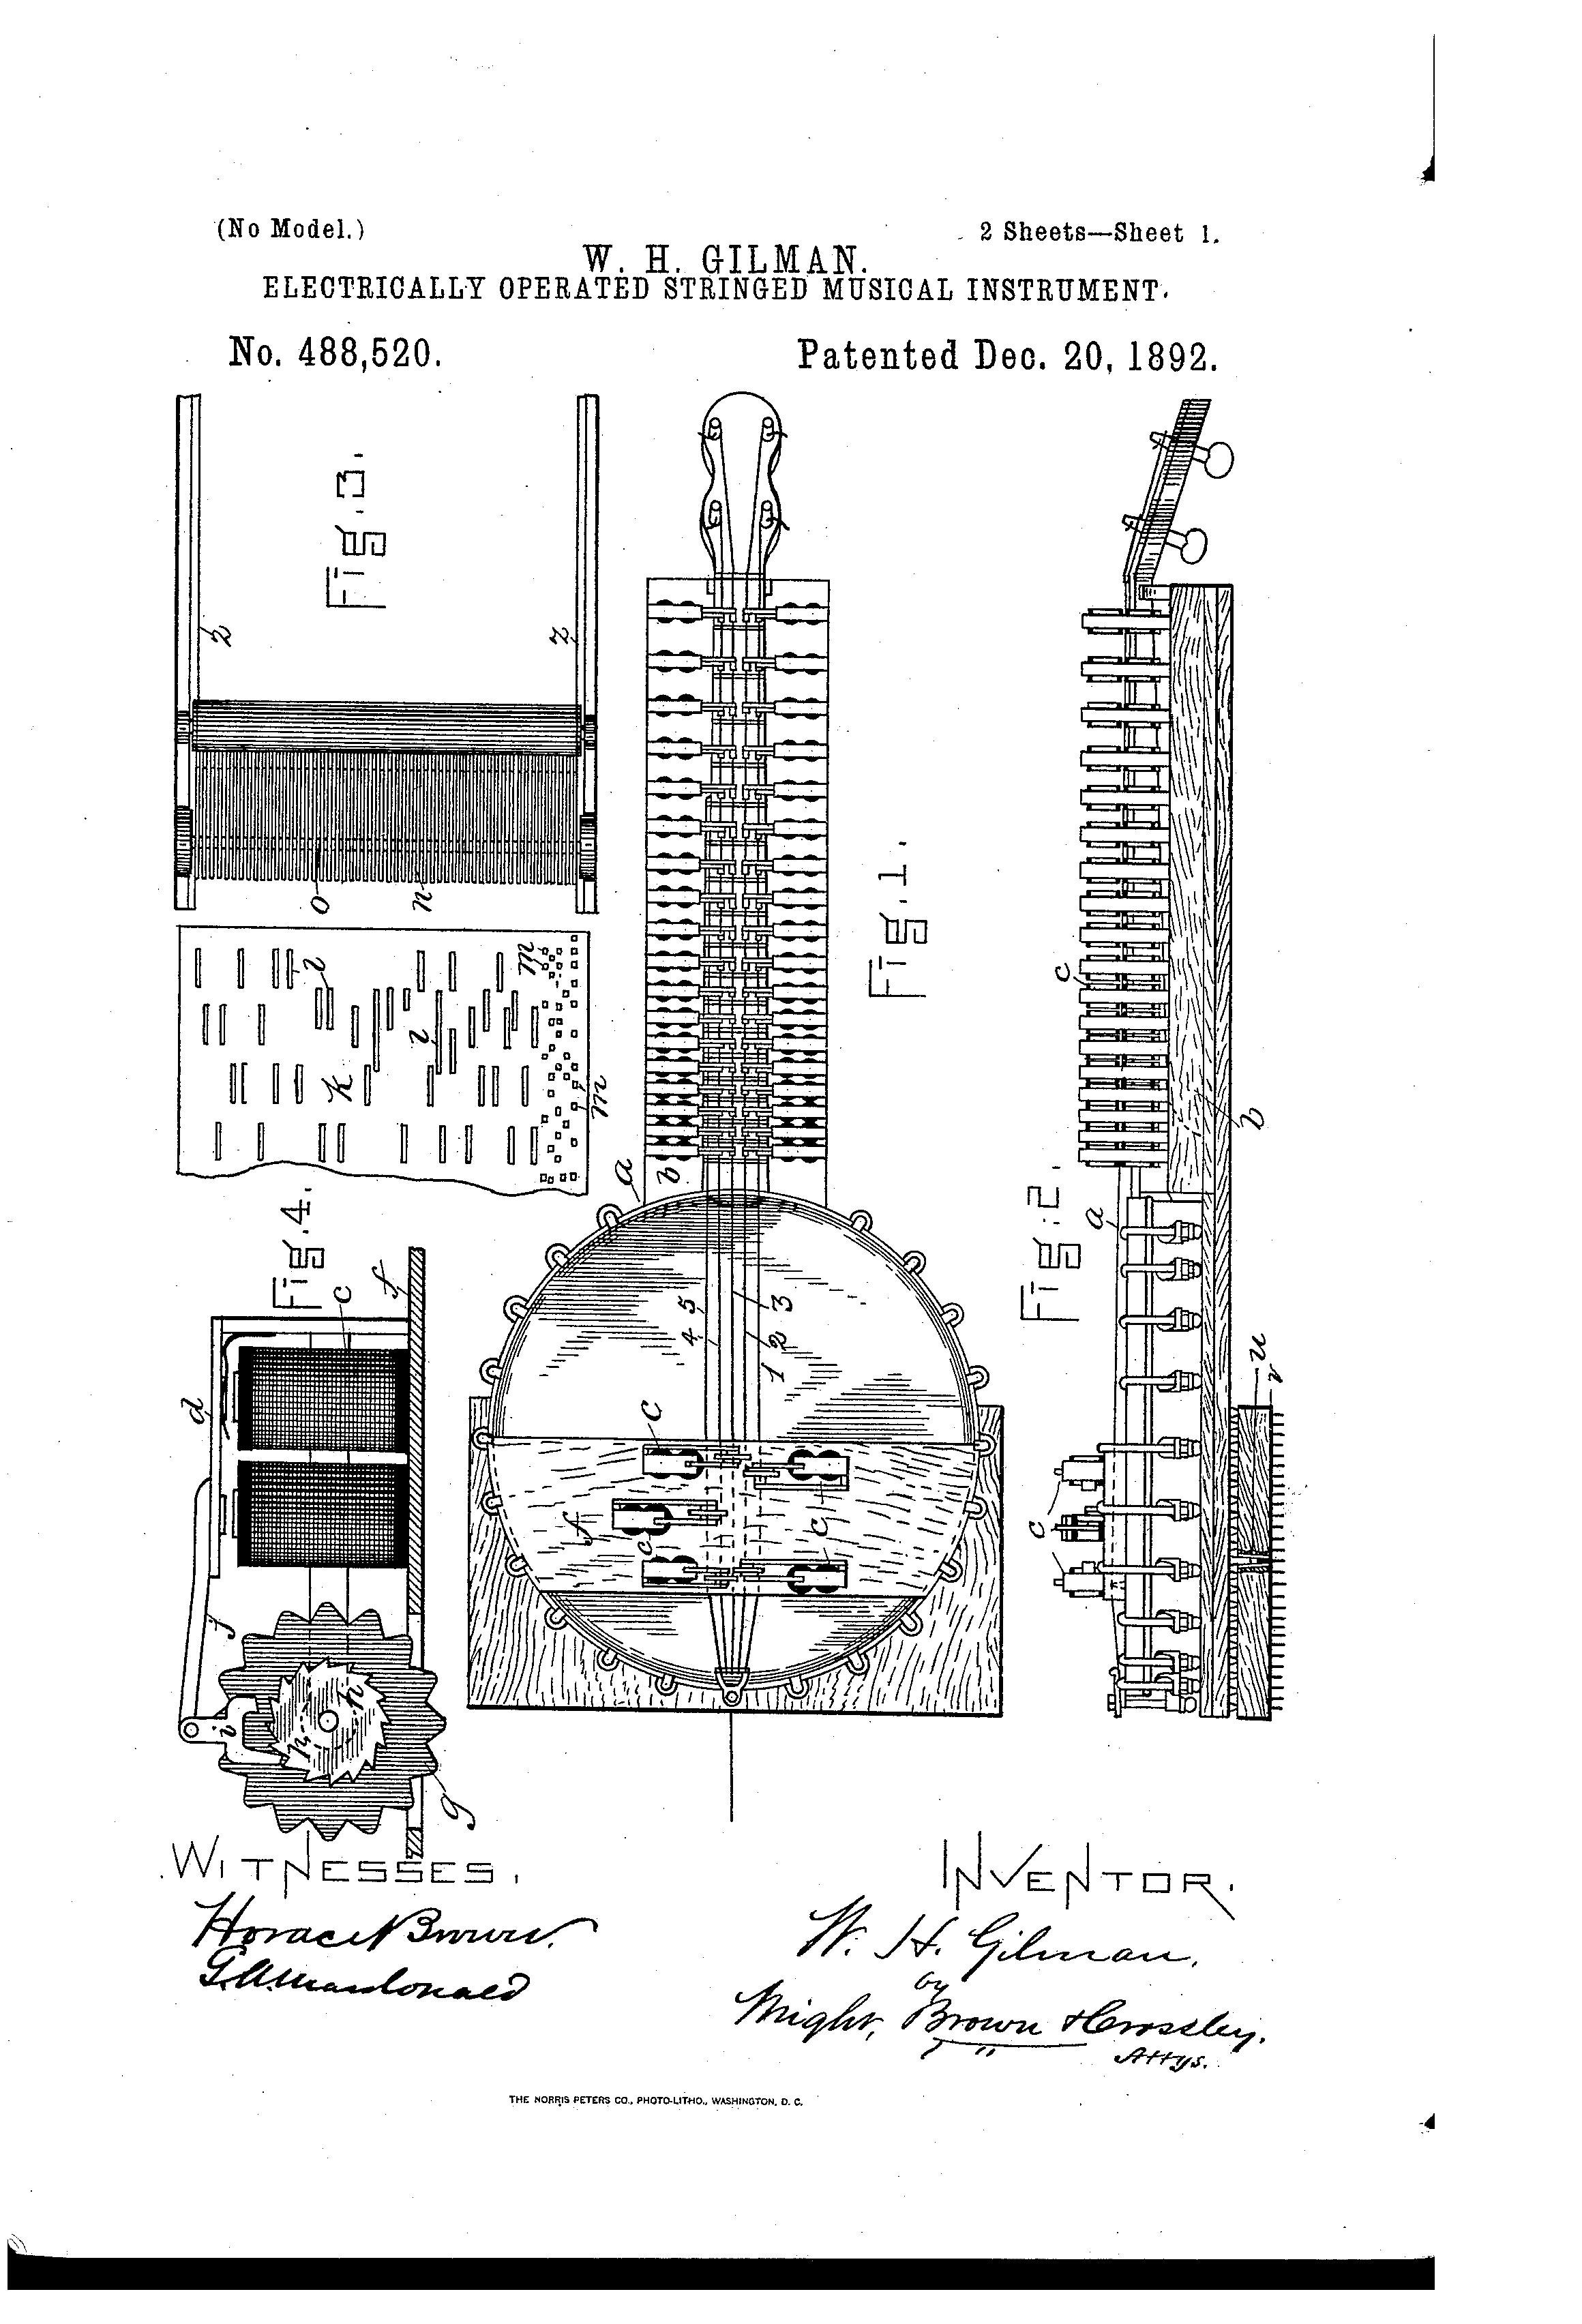
\includegraphics[scale=0.18]{images/patente1.png}
        \end{subfigure}
        \begin{subfigure}{0.3\textwidth}
            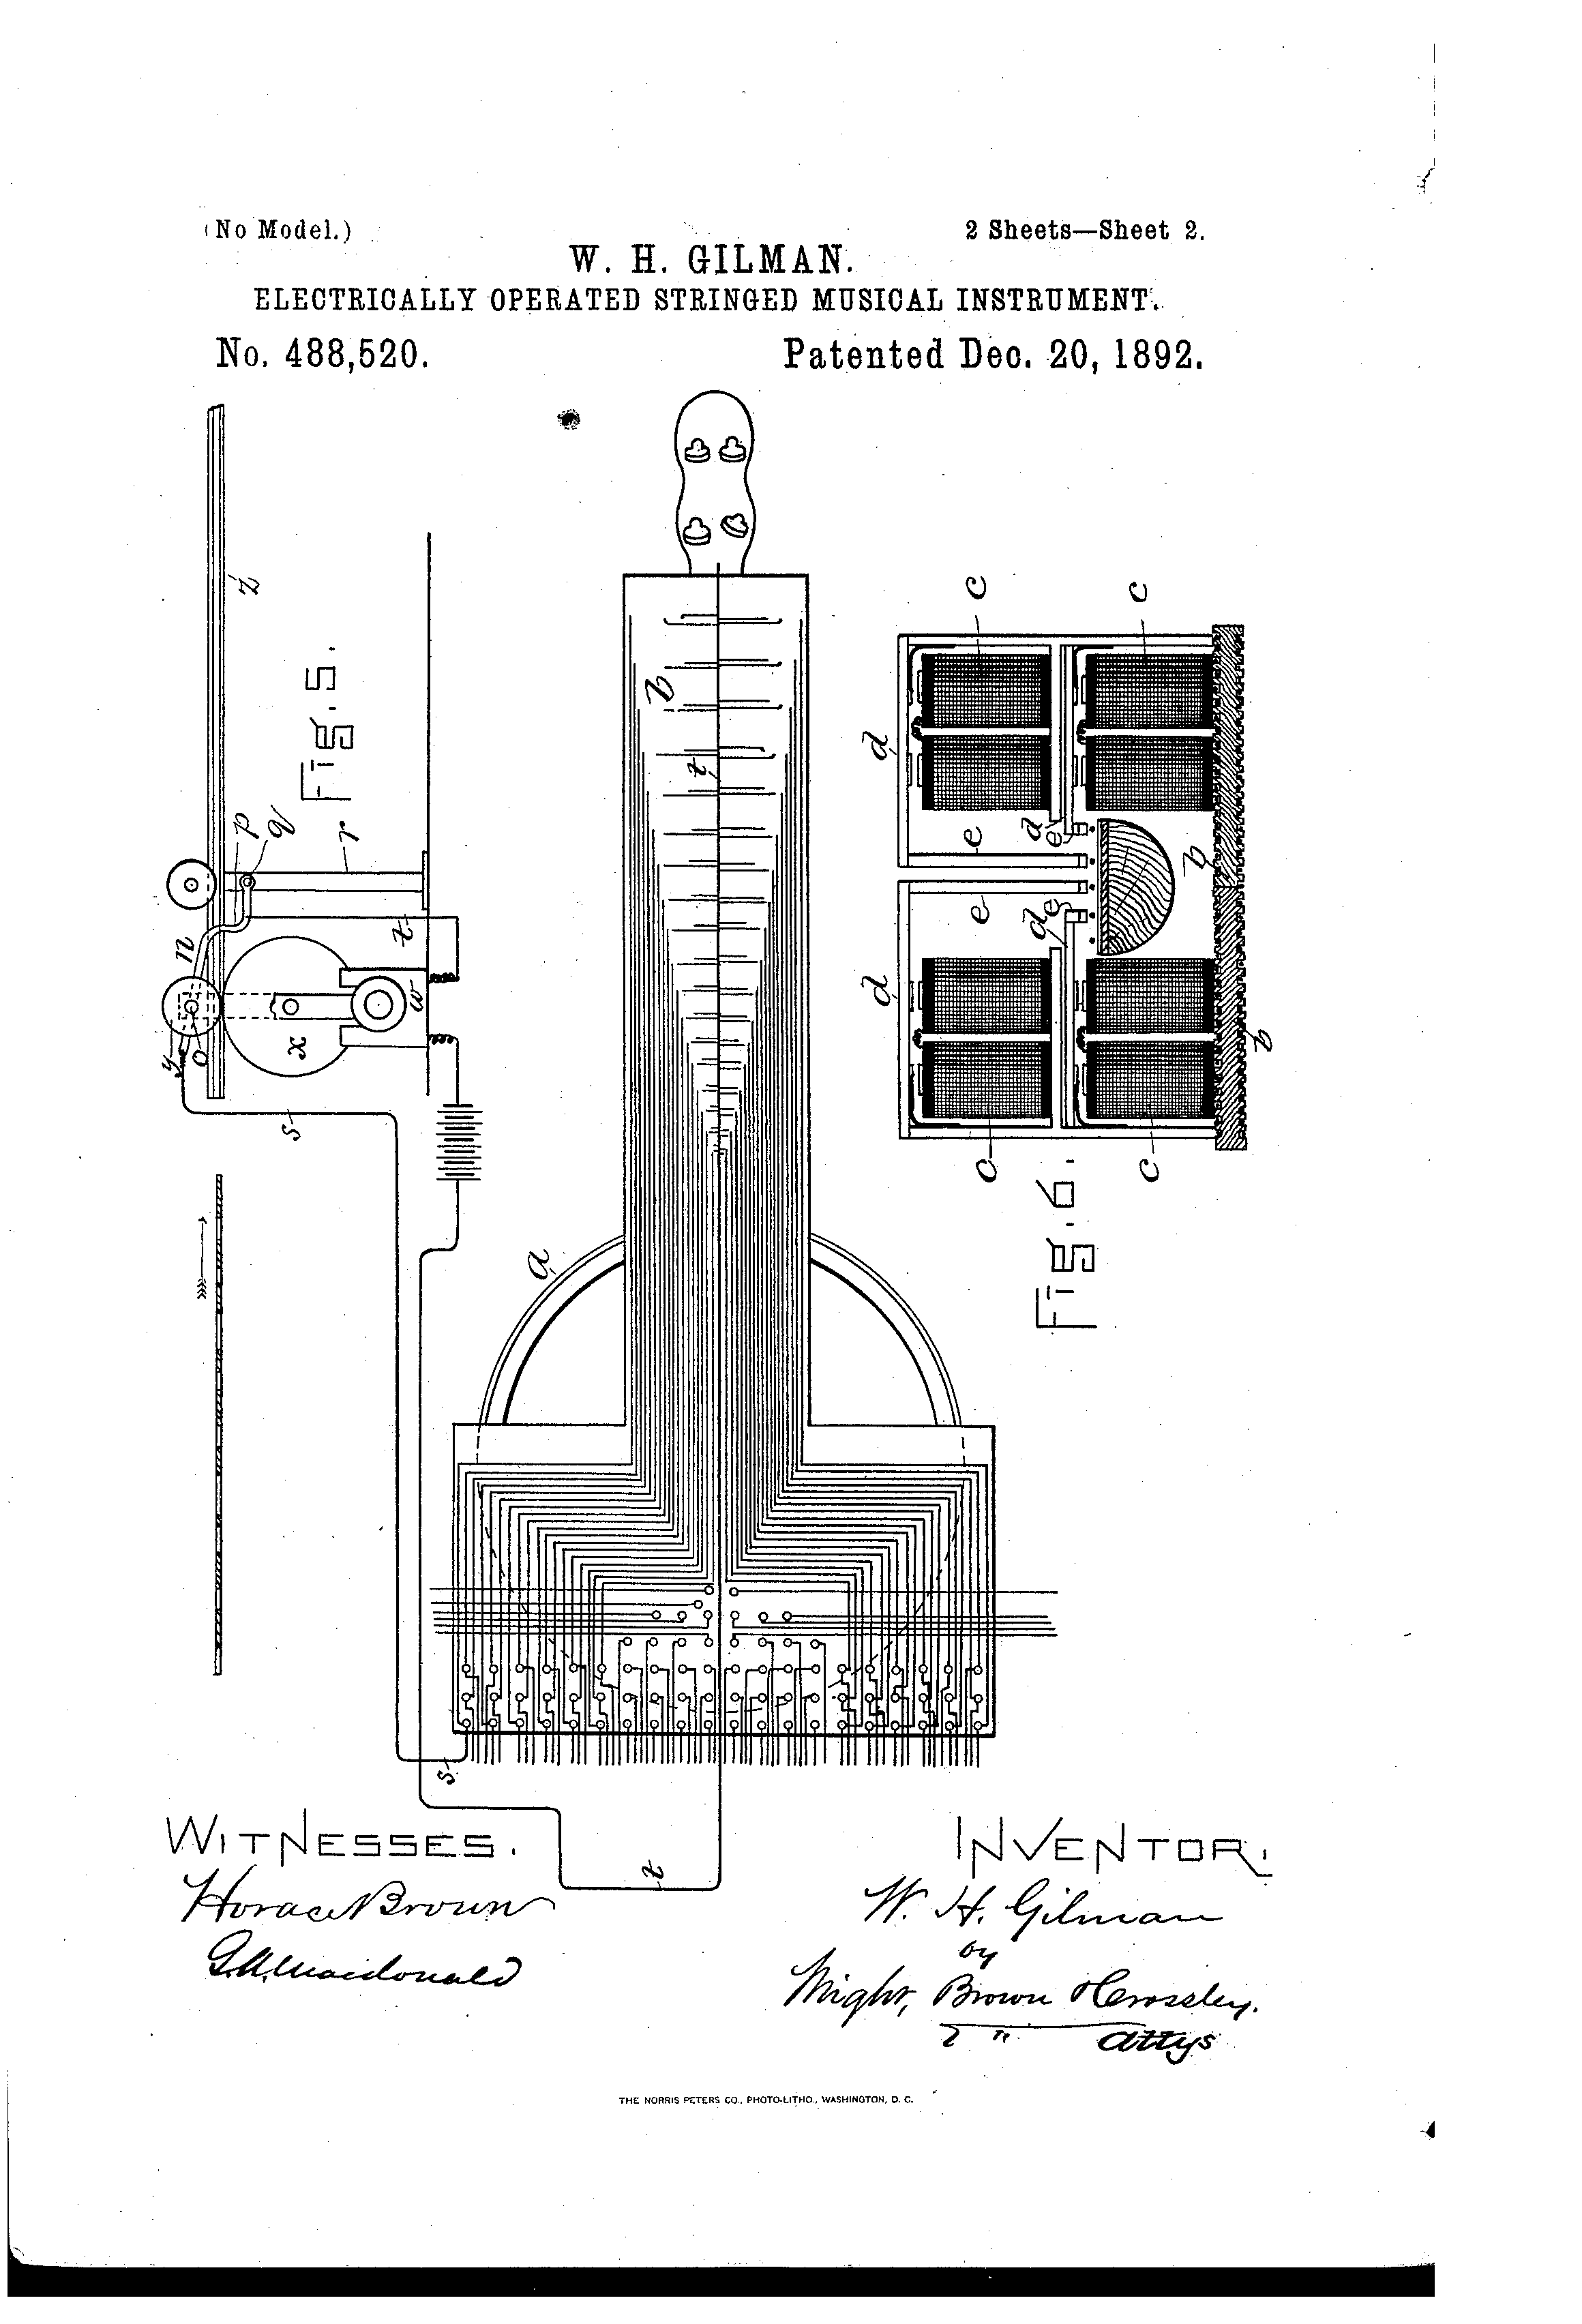
\includegraphics[scale=0.18]{images/patente2.png}
        \end{subfigure}
    \end{center}
    \vspace{-5pt}
    \caption{La patente de W.H. Gilman}
\end{figure}

Pero el desarrollo de la guitarra eléctrica empezaría con más fuerza en la década de 1920, llevada por la necesidad de los guitarristas de Big Bands de ser un instrumento principal y no ser relegado a ser un acompañamiento de los instrumentos de viento de cobre. En esta década empezaría la experimentación de varias compañías para poder amplificar el sonido de la guitarra. \\

Gibson empezaría a experimentar con el diseñador Lloyd Loar, quien fue contratado en 1919 y durante 5 años lograría llevar a cabo varios experimentos con sistemas electroestáticos, pero sin resultados óptimos, siendo despedido en 1924 después de que la compañía no viera un potencial comercial en estos. \\

\begingroup
\setlength{\intextsep}{0pt}%
\setlength{\columnsep}{0pt}%

\begin{wrapfigure}{r}{0.37\textwidth}
    \centering
    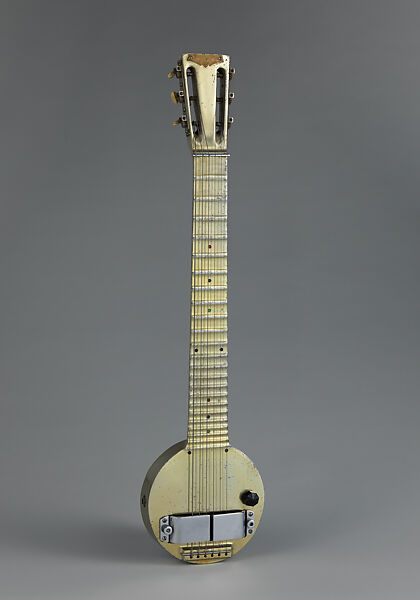
\includegraphics[width=0.27\textwidth]{images/frying_pan.jpg}
    \vspace{-5pt}
    \caption{Frying Pan}
\end{wrapfigure}

George Beauchamp y Adolph Rickenbacker (quienes fundarían la compañía Rickenbacker tiempo después) empezarían en Los Angeles, California a experimentar con pastillas electromagnéticas, que consistían en dos imanes en forma de herradura alrededor de las cuerdas. Con esta invención, en 1932 lanzarían al mercado la “Frying Pan”, una guitarra de regazo de acero hawaiana eléctrica. Aplicarían por la patente en 1932 pero hasta 1937 quedo registrada, lo cual permitió que otras empresas empezaran a desarrollar y vender guitarras eléctricas.

\endgroup

\section{El nacimiento de la ES-150}

Después de la Gran Depresión, el éxito que tiene Rickenbacker con su “Frying Pan” lleva a Gibson a investigar cómo pueden amplificar el sonido sin infligir las patentes existentes y llegar a su propia versión de la amplificación del sonido de sus instrumentos.\\

\begingroup
\setlength{\intextsep}{0pt}%
\setlength{\columnsep}{0pt}%

\begin{wrapfigure}{l}{0.5\textwidth}
    \centering
    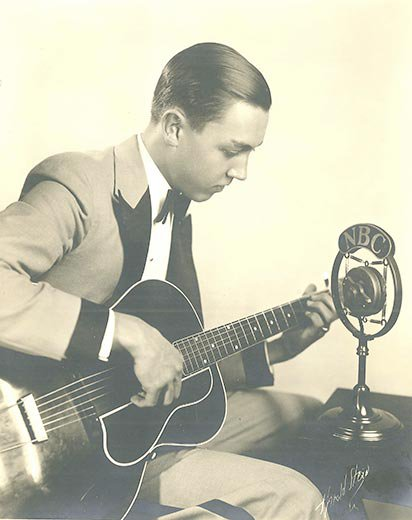
\includegraphics[width=0.4\textwidth]{images/rey_alvino.jpg}
    \vspace{-5pt}
    \caption{Rey Alvino tocando la Gibson L-5}
\end{wrapfigure}

En 1934, el gerente general Guy Hart, viendo que no hay expertos dentro de la compañía que puedan llevar a cabo experimentos con la amplificación de las guitarras, coopera con la compañía de Chicago Lyon \& Healy, y envía allí al ingeniero John Kutalek para que empiece el desarrollo de la guitarra eléctrica. Además, Hart también recluta a Alvino Rey, guitarrista de regazo de acero conocido por su uso de la Frying Pan.\\

Pese a que Rey ayudo dando detalles valiosos sobre la construcción de la guitarra eléctrica, los experimentos realizados en Chicago no dieron frutos y el proyecto seria movido a la fábrica de Gibson en Michigan para seguir con los experimentos; ya en la fábrica, el proyecto seria tomado por Walter Fuller.\\

\endgroup

Parte del problema de crear una pastilla que funcionara, era que Kutalek quería replicar la pastilla de Rickenbacker, pero sin infringir el uso de la patente. Entonces, Fuller utilizo métodos para investigar cómo se podía enrollar la bobina, el uso de diferentes imanes y el tamaño de las pastillas, ya que era algo nuevo a lo que los ingenieros se estaban enfrentando intentándolo a prueba y error.\\

\begingroup
\setlength{\intextsep}{0pt}%
\setlength{\columnsep}{0pt}%

\begin{wrapfigure}{r}{0.45\textwidth}
    \centering
    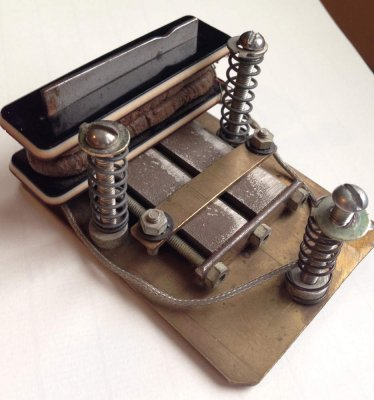
\includegraphics[width=0.35\textwidth]{images/pickup.jpg}
    \vspace{-5pt}
    \caption{Pastilla de barra}
\end{wrapfigure}

Entonces en 1935, Gibson encontraría su manera de hacer una pastilla para su guitarra eléctrica, siendo el primer modelo en usarla una guitarra eléctrica hawaiana. Esta pastilla, comúnmente llamada “pastilla de barra”, se caracteriza por tener una bobina atravesada con una platina metálica que sirve como polo para todas las cuerdas, la cual tenía tres cortes; dos imanes planos (4.5’’ x 1.25’’ x 0.375’’) puestos perpendicularmente debajo de la bobina, y cuando se instalaba no se veía, solo la parte superior de la platina.\\

\endgroup

Las primeras versiones de la pastilla estaban hechas de níquel y acero, donde la bobina era enrollada con 4000 vueltas de alambre calibre 38 donde se obtenía una resistencia de $4000 \Omega$. Las siguientes versiones estarían hechas de cobalto y acero, con la bobina enrollada con 10000 vueltas de alambre calibre 42, generando una resistencia de $8000 \Omega$. \\

En febrero de 1936, Gibson aplicaría por la patente US2087106A, con la cual registra su modelo de pastilla y la cual utilizaría en sus demás instrumentos.\\

\begin{figure}[h]
    \begin{center}
        \begin{subfigure}{0.3\textwidth}
            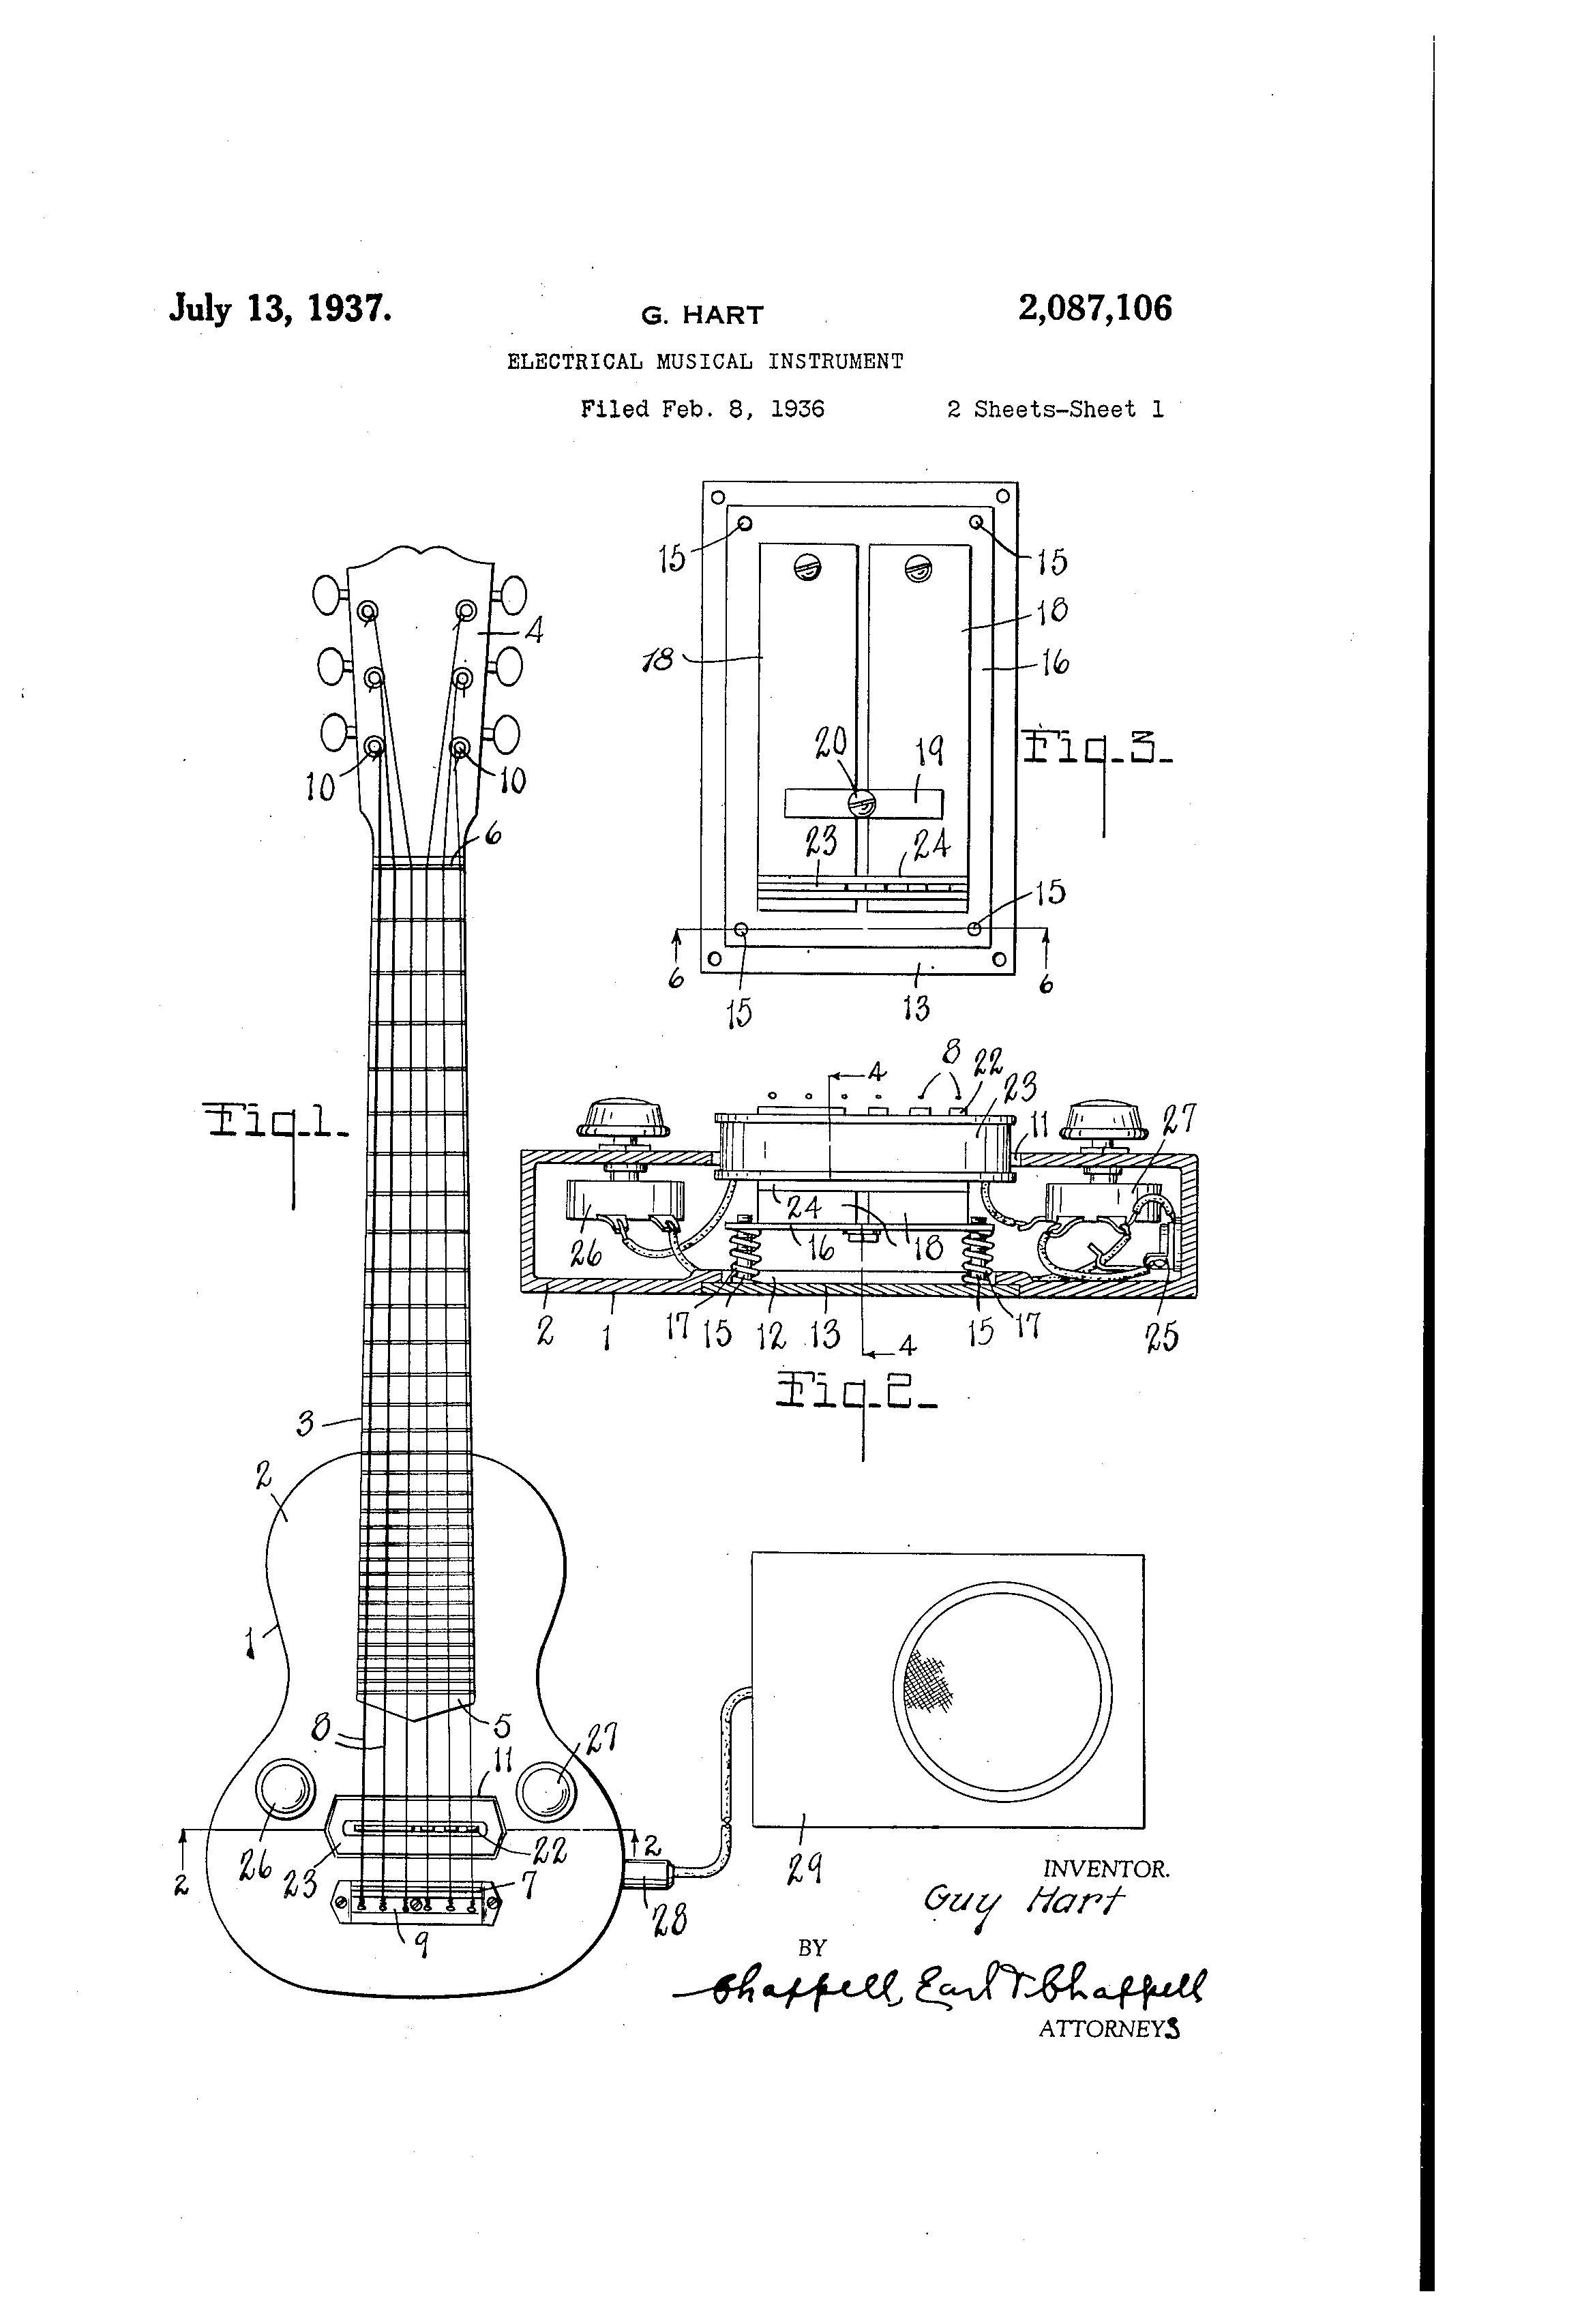
\includegraphics[scale=0.18]{images/patente3.png}
        \end{subfigure}
        \begin{subfigure}{0.3\textwidth}
            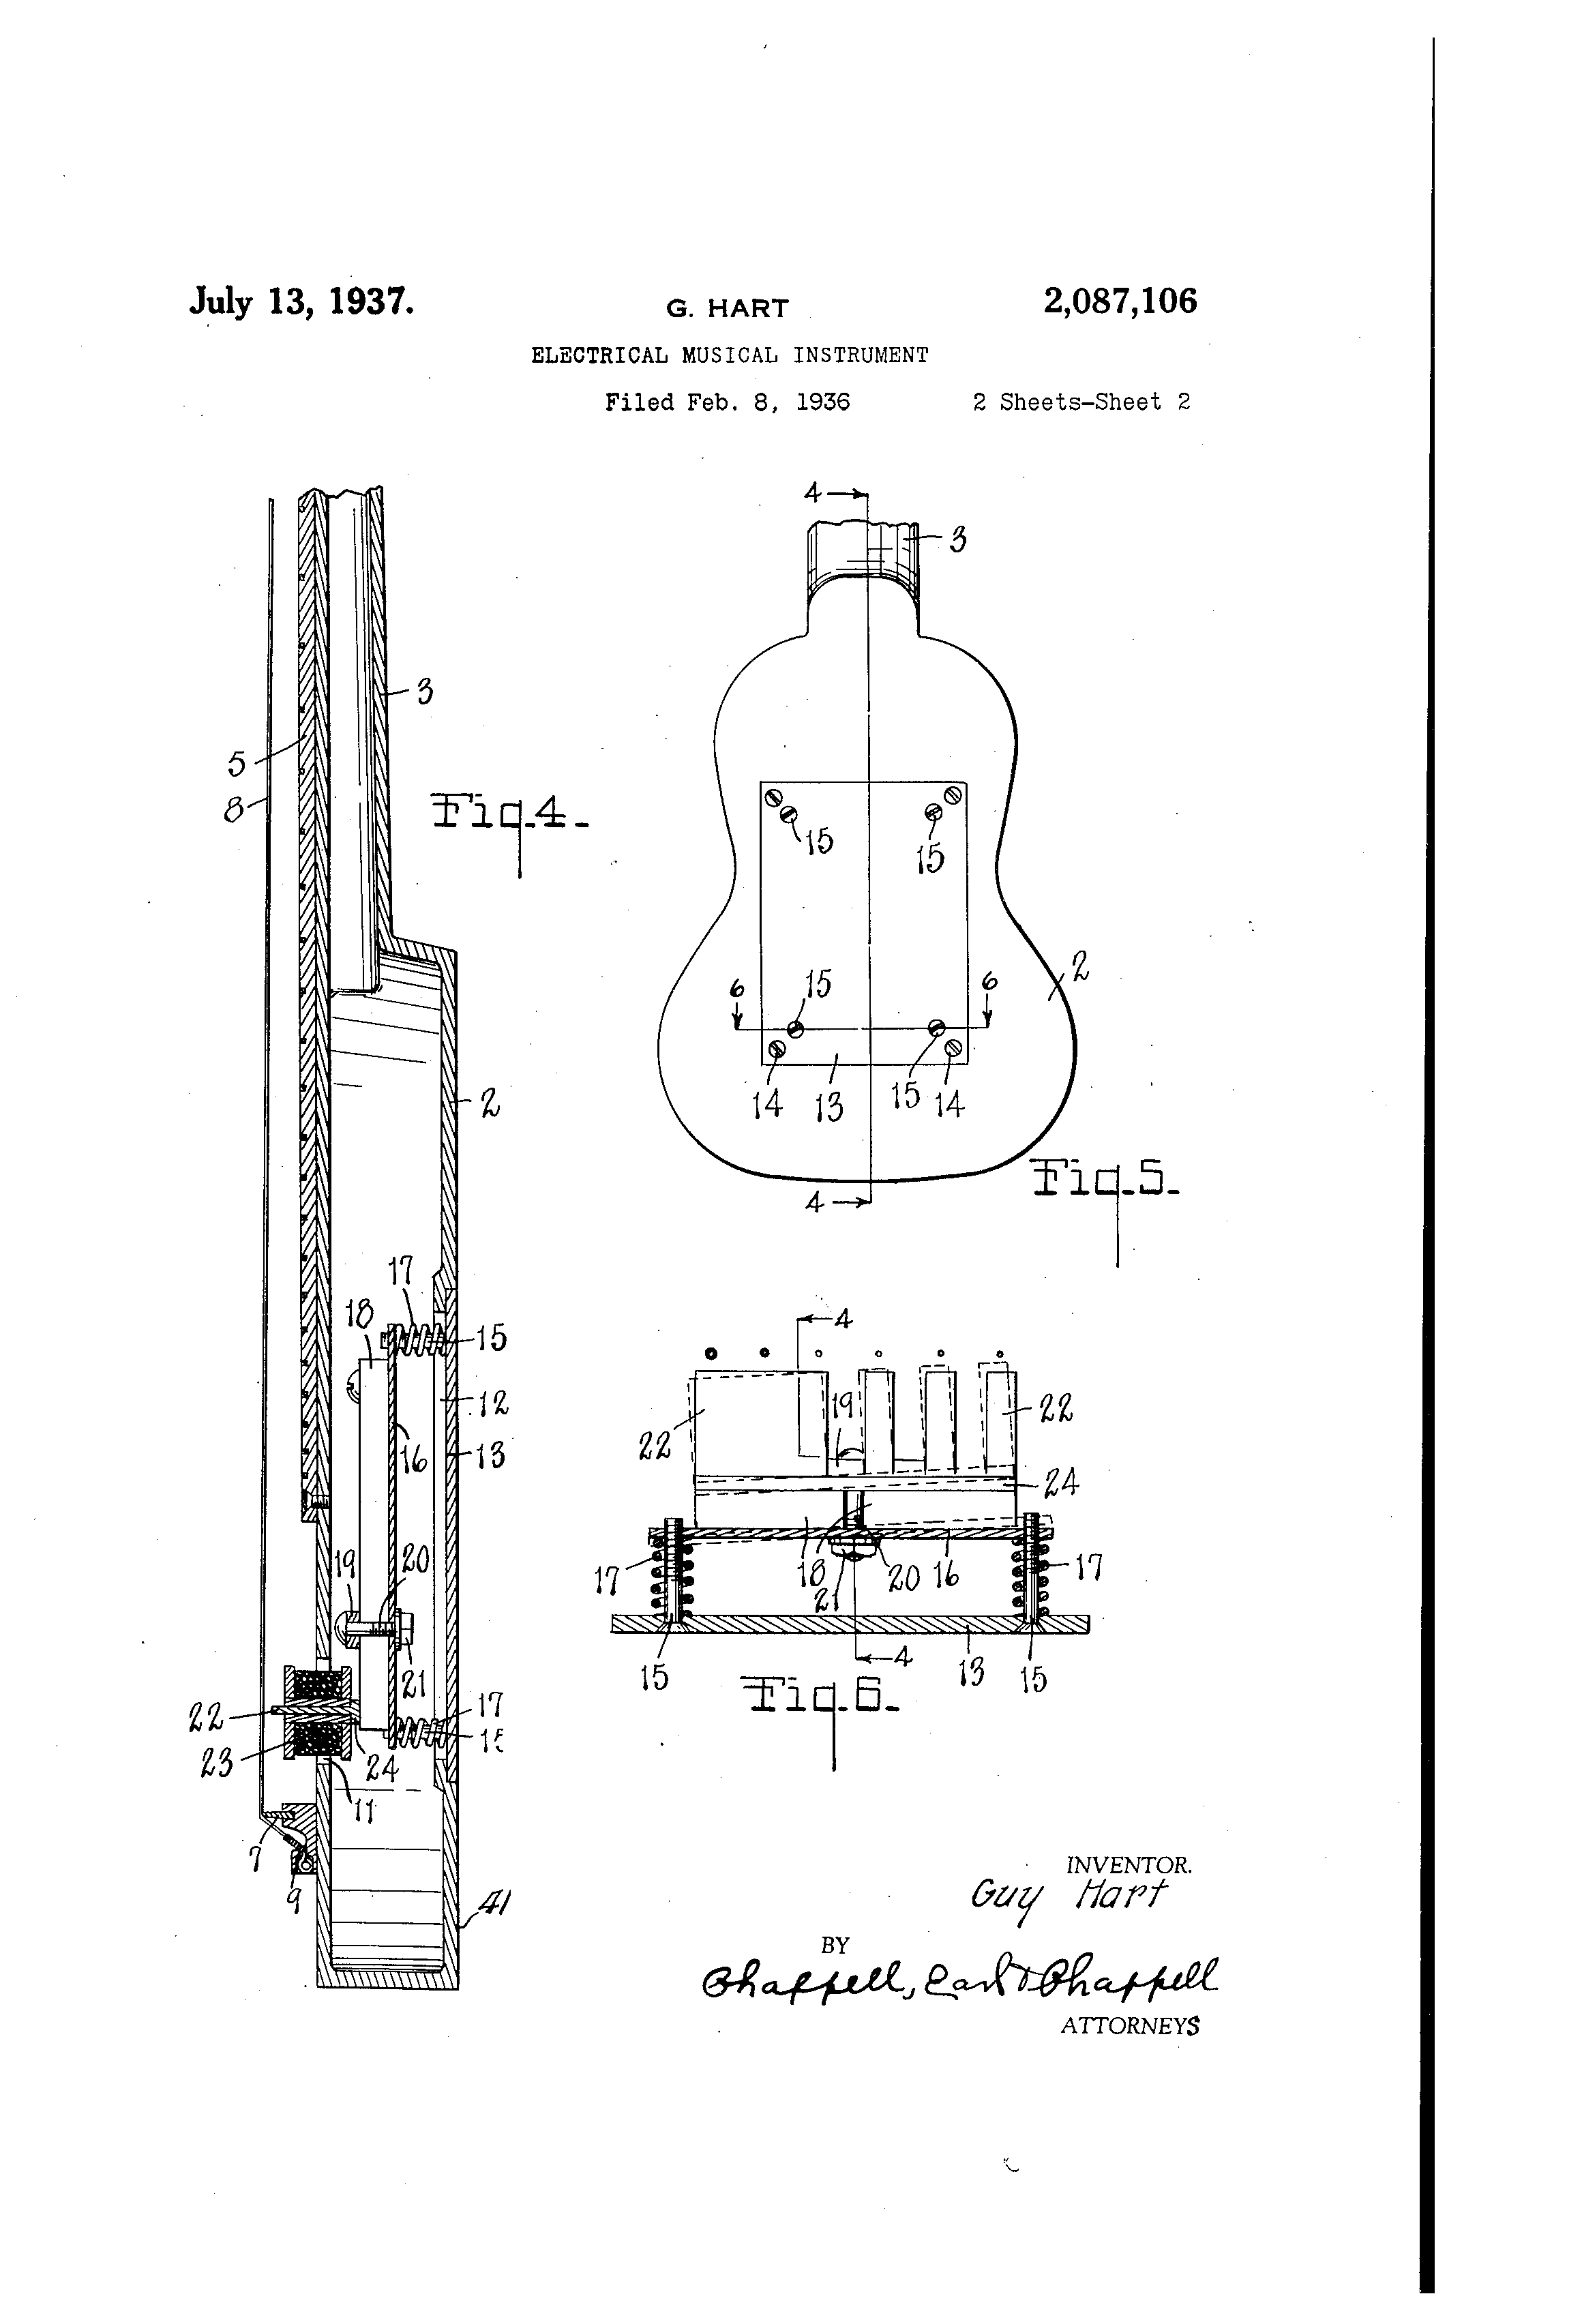
\includegraphics[scale=0.18]{images/patente4.png}
        \end{subfigure}
    \end{center}
    \vspace{-5pt}
    \caption{La patente de la guitarra hawaiana Gibson}
\end{figure}

A mediados de 1396, Gibson lanzaría al mercado el modelo de guitarra ES-150, su primera guitarra española eléctrica. Con un valor de US \$150 (con el amplificador incluido) y con el eslogan: “Otro milagro de la guitarra por Gibson – un tono autentico, sin distorsión, amplificada por electricidad”.\\

\begingroup
\setlength{\intextsep}{12pt}%
\setlength{\columnsep}{0pt}%

\begin{wrapfigure}{l}{0.45\textwidth}
    \centering
    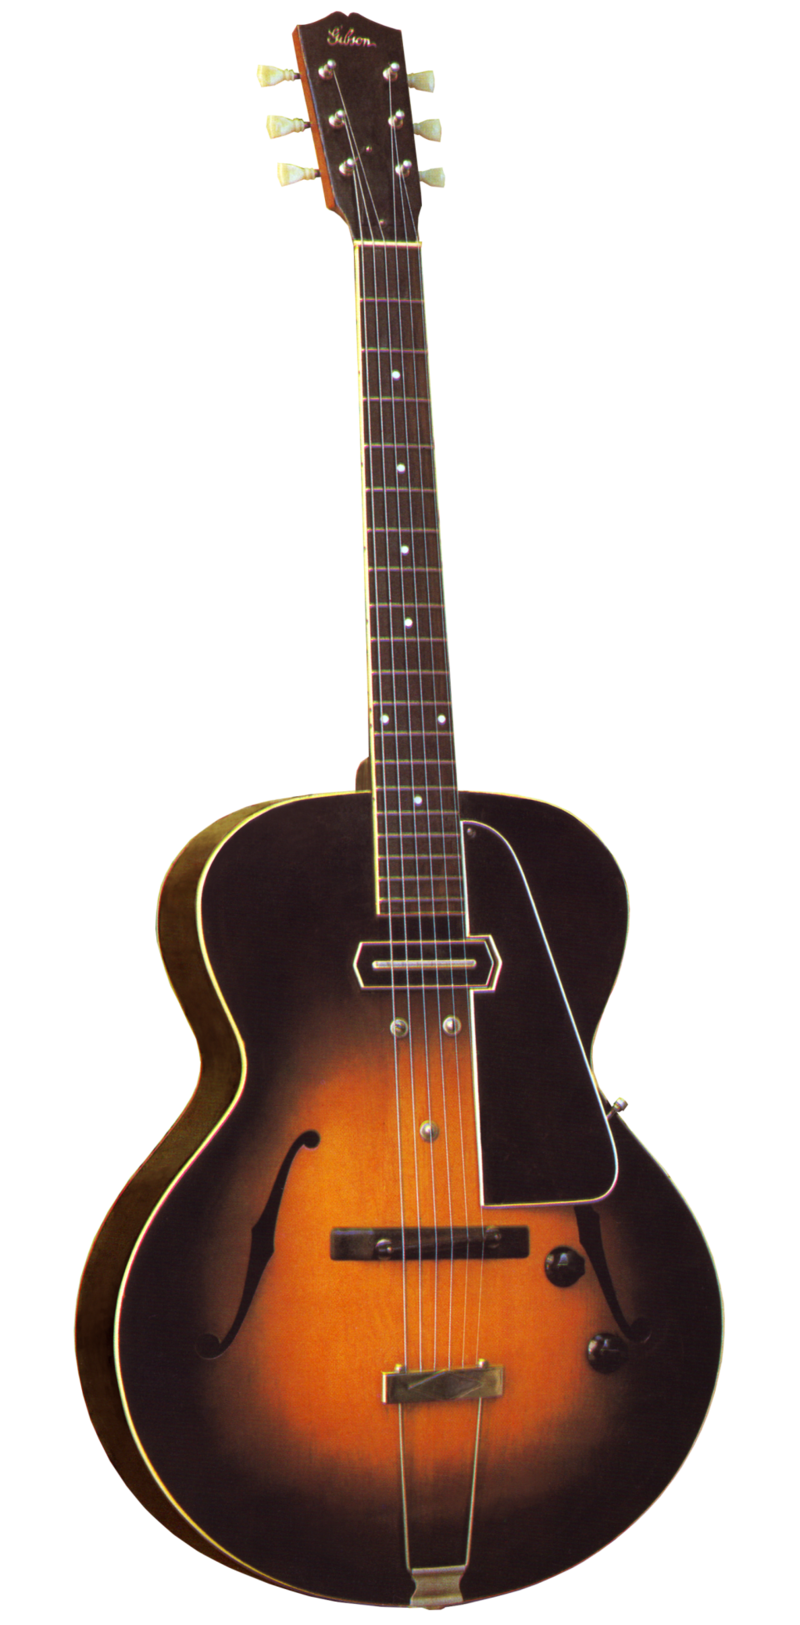
\includegraphics[width=0.35\textwidth]{images/es-150.png}
    \vspace{-5pt}
    \caption{Gibson ES-150}
\end{wrapfigure}

Las caracteristicas de la Gibson ES-150 son:

\begin{itemize}
    \item Escala: 24 \(\frac{3}{4}\)'
    \item Cuerpo: Cuerpo hueco de 16 \(\frac{3}{4}\)' de ancho con una tapa superior de arco de abeto macizo, aros y fondo de arce sólido.
    \item Unión: Mástil encolado.
    \item Mástil: Caoba.
    \item Diapazón: Palisandro con incrustaciones de puntos perlados.
    \item Puente: Ébano tipo arco de altura ajustable.
    \item Color: Sunburst.
\end{itemize}

Pero la ES-150 no tenía la pastilla usada en la guitarra hawaiana, sino que contaba con una pastilla un poco más pequeña y la platina metálica era completa, no con los tres cortes.\\

\endgroup

\section{Influencia}

Aunque la producción de la ES-150 empezó en 1936, solo hasta 1937 fue distribuida en masa. Cuando se volvió disponible, capto la atención de los guitarristas que ya habían experimentado con la amplificación por electricidad.\\

\begingroup
\setlength{\intextsep}{0pt}%
\setlength{\columnsep}{0pt}%

\begin{wrapfigure}{r}{0.43\textwidth}
    \centering
    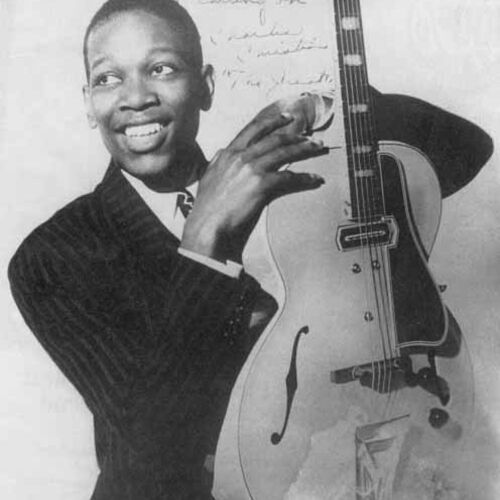
\includegraphics[width=0.33\textwidth]{images/cc.jpg}
    \vspace{-5pt}
    \caption{Charlie Christian}
\end{wrapfigure}

El primer guitarrista, Eddie Durham, reconocido como el primero en grabar solos en 1938 con su banda, Kansas City Six. Además, convertiría a la guitarra al banjoista Floyd Smith y le presentaría la guitarra a Charlie Christian, el primer gran exponente de la guitarra eléctrica y del modelo ES-150.\\

Charlie Christian nacido en Texas en 1916, fue uno de los primeros musicos de Jazz que adoptaría la ES-150 como su instrumento principal mientras tocaba con la banda de Benny Goodman. Gracias a esto, la guitarra dejaría de ser el instrumento que era y encontraría su voz como la conocemos hoy en día. Charlie predicaba tocar la guitarra en solitario, decía: “Practiquen solos, toquen en una sola cuerda, y más que nada, salven algunos centavos para amplificar su instrumento.”\\

\endgroup

Charlie moriría en 1942 por problemas de salud, pero dejando un legado inigualable. La pastilla que tiene la ES-150 son llamadas CC pickups, en tributo a uno de los pioneros de la forma de tocar la guitarra actualmente.\\

\begingroup
\setlength{\intextsep}{0pt}%
\setlength{\columnsep}{0pt}%

\begin{wrapfigure}{l}{0.5\textwidth}
    \centering
    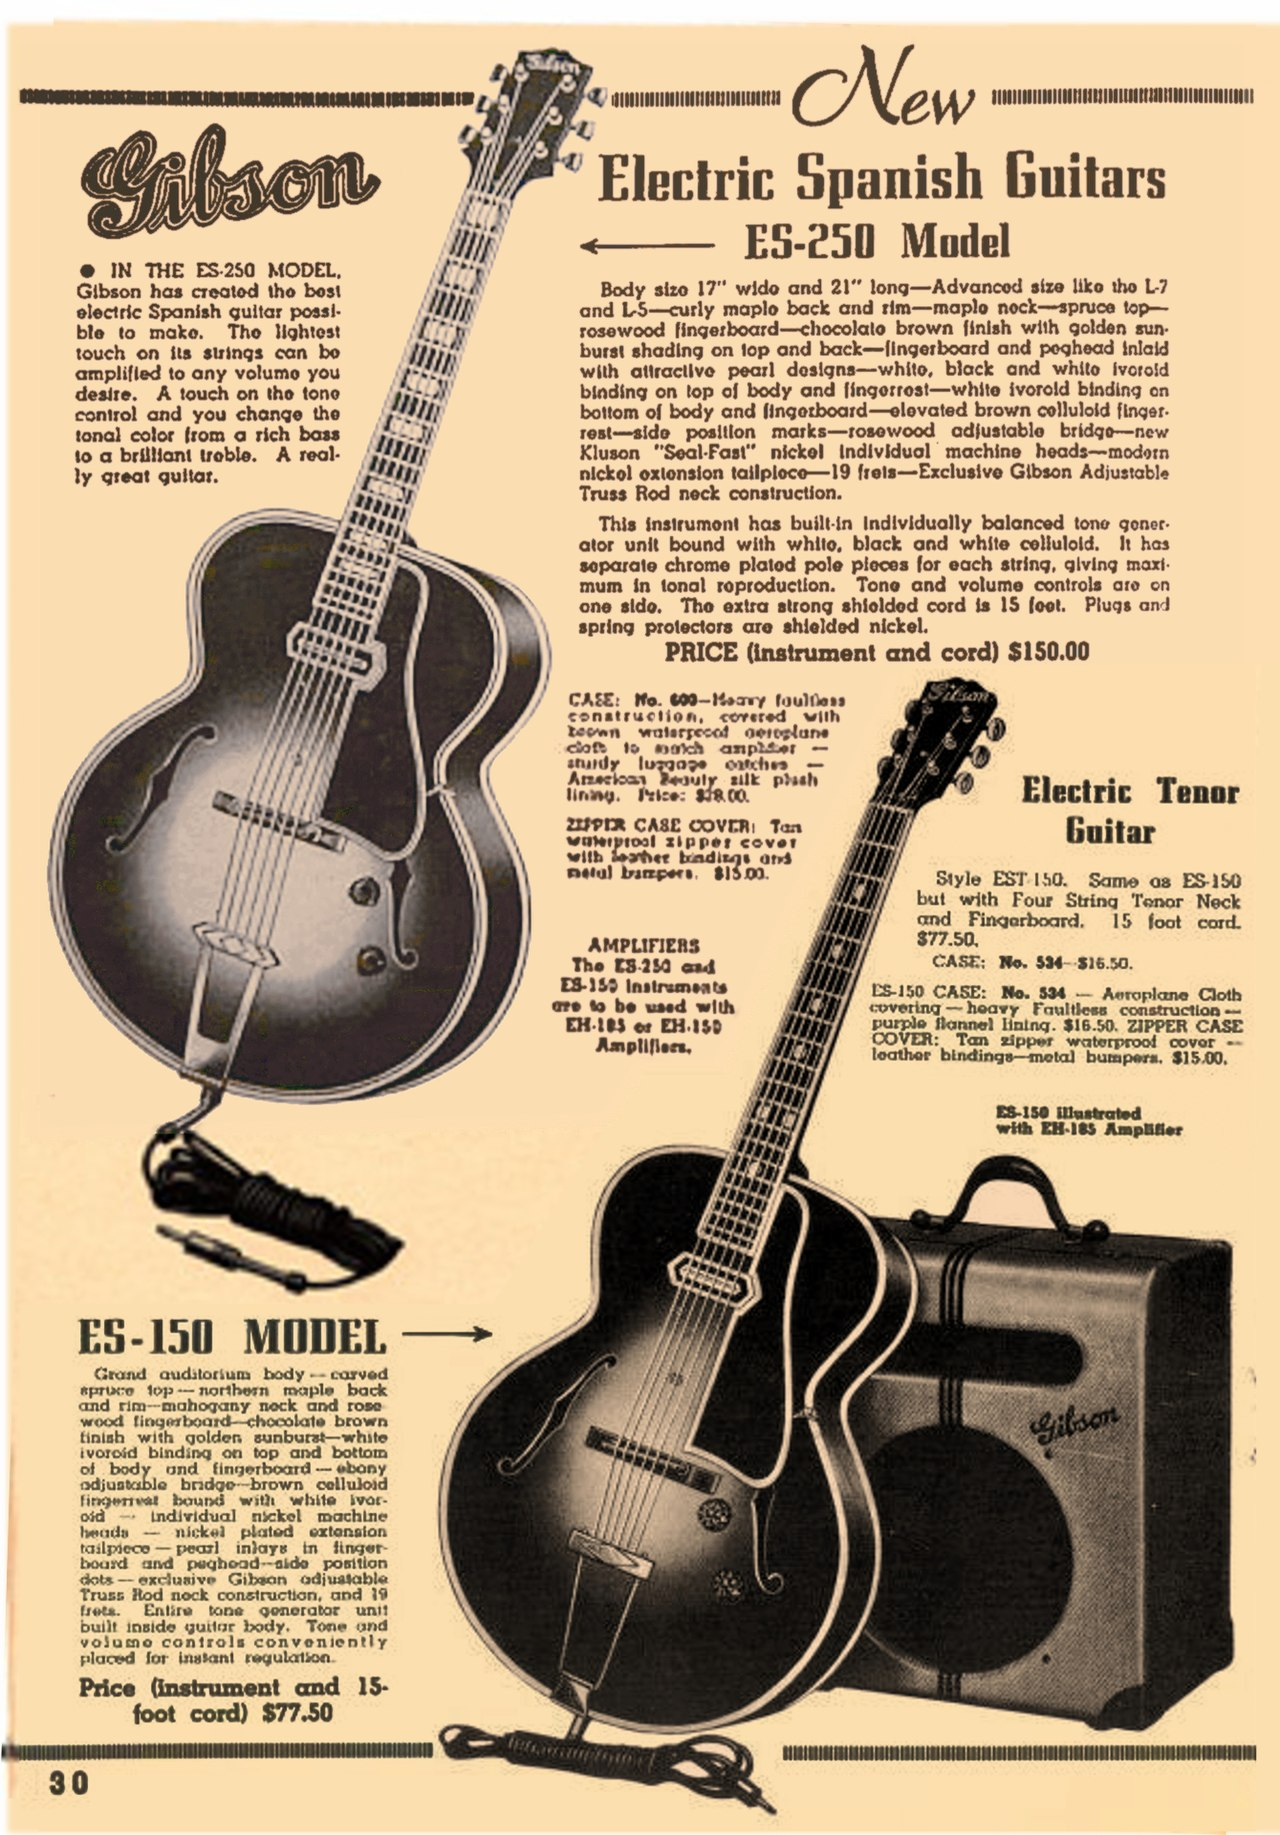
\includegraphics[width=0.4\textwidth]{images/promo.jpg}
    \vspace{-5pt}
    \caption{Propaganda de la ES-250 y ES-150}
\end{wrapfigure}

La ES-150 le abrió las puertas a que Gibson desarrollara la línea de guitarras ES, donde estarían guitarras eléctricas que se vendían desde los US \$100 y con diferentes dimensiones y especificaciones. Entre ellas encontramos la ES-100, una guitarra de 14 \(\frac{3}{4}\)' de escala que costaba US \$100 con su amplificador, estuche y cuerdas; también se vendía la ES-250, una versión mejorada de la ES-150, donde se promocionaba como ‘La mejor guitarra eléctrica posible para hacer’, donde contaba con un generador individual de tono balanceado, donde la pastilla tenía 6 cortes para cada una de las cuerdas. Cuando salió la ES-250 fue adoptaba por muchos de los guitarristas de la época, incluyendo al legendario Charlie Christian.\nocite{*}

\endgroup

\printbibliography[
title={Bibliografía}
]

\end{document}